\documentclass[reprint,amsmath,amssymb,aps]{revtex4-2}

\usepackage{graphicx}
\usepackage{dcolumn}
\usepackage{bm}
\usepackage{hyperref}

\begin{document}

\title{Ultra-High-Density Matter in Active Galactic Nuclei: \\
Constraints from Multi-Messenger Observations}

\author{[Author Names]}
\affiliation{[Institution]}

\date{\today}

\begin{abstract}
[Abstract text describing UHDM production in AGN jets, EFT calculations,
GRMHD simulations, and multi-messenger constraints from Fermi-LAT,
IceCube, and Pierre Auger Observatory.]
\end{abstract}

\maketitle

\section{Introduction}
[Introduction content]

\section{GRMHD Acceleration Mechanism}
[Description of magnetically-dominated jet acceleration]

\section{EFT Production Cross Sections}
[Effective field theory calculations and parton-level processes]

\section{Monte Carlo Parameter Scan}
[MCMC methodology using emcee with 10^6 samples]

\section{Multi-Messenger Constraints}
\subsection{Fermi-LAT Gamma-Ray Limits}
\subsection{IceCube Neutrino Constraints}
\subsection{Pierre Auger UHECR Data}

\section{Results}
\begin{figure}
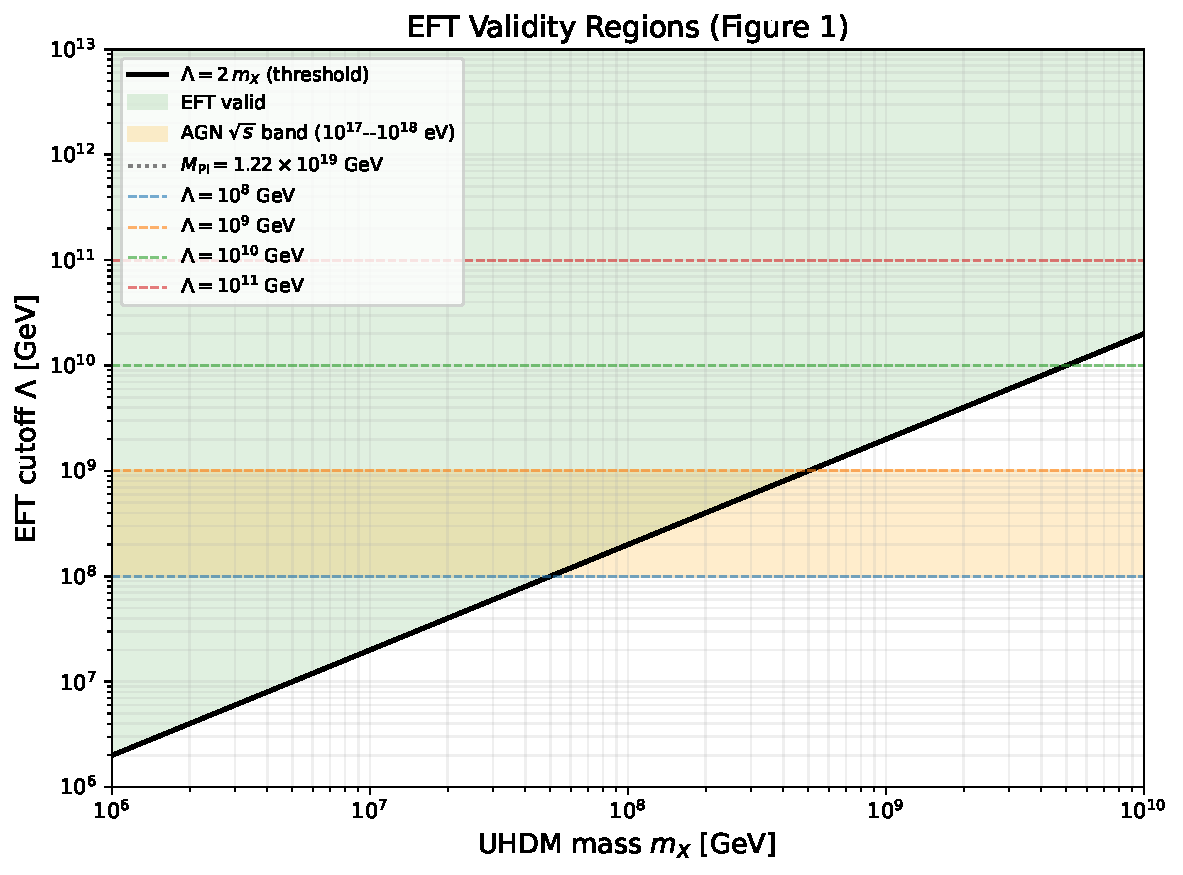
\includegraphics[width=\columnwidth]{../figures/fig1_eft_validity_corrected.pdf}
\caption{EFT validity cutoff analysis.}
\label{fig:eft_validity}
\end{figure}

\begin{figure}
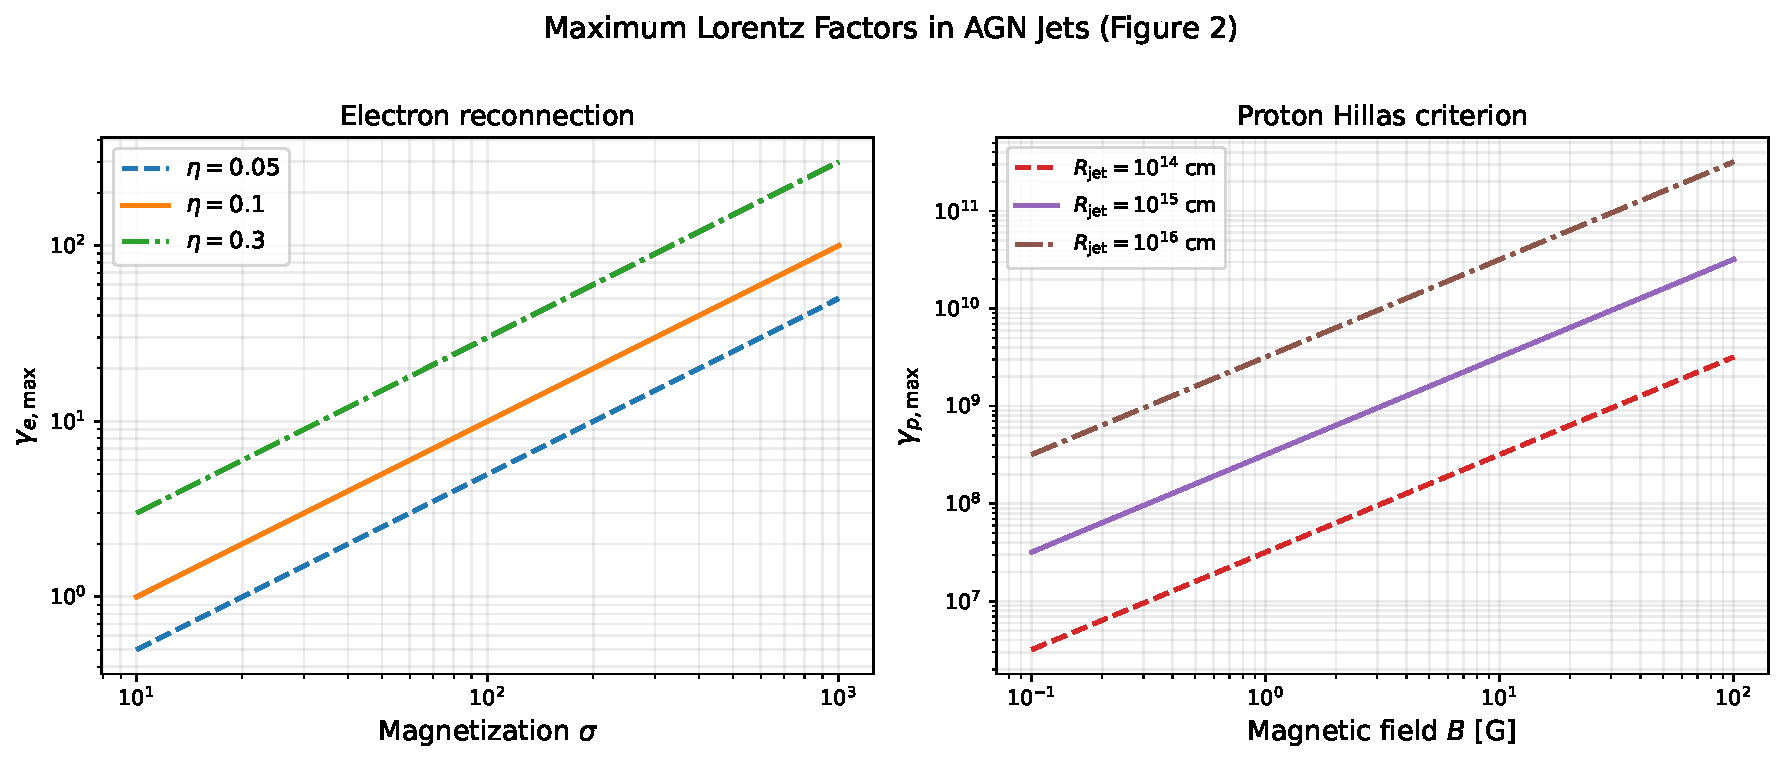
\includegraphics[width=\columnwidth]{../figures/fig2_gamma_max.pdf}
\caption{Maximum Lorentz factors in GRMHD simulations.}
\label{fig:gamma_max}
\end{figure}

\begin{figure}
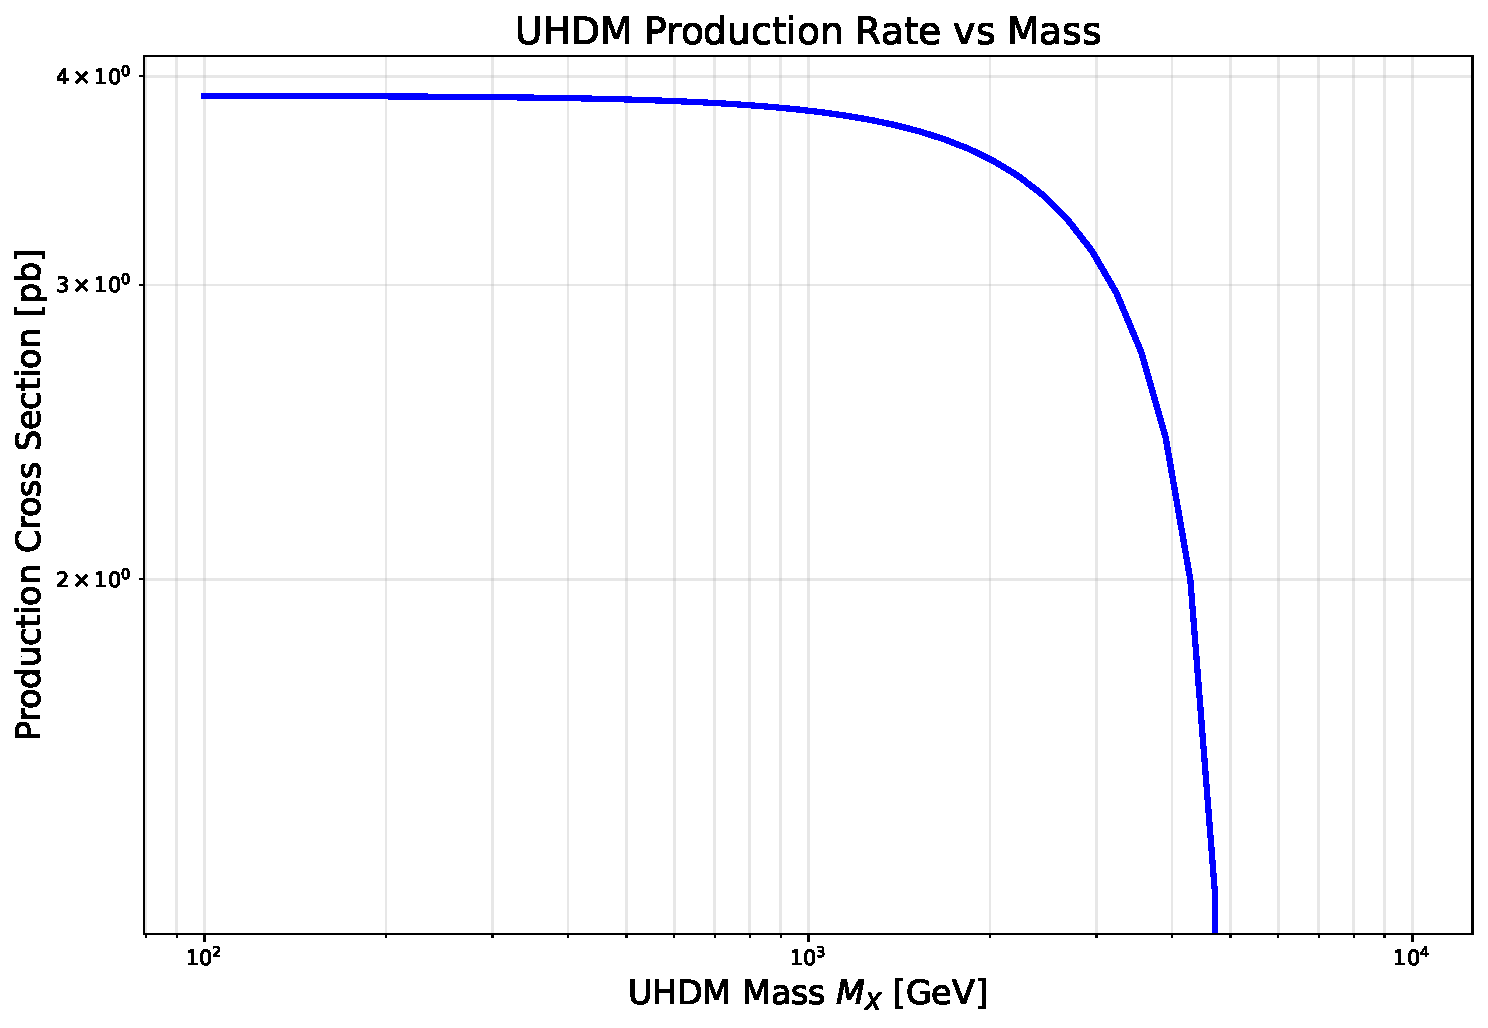
\includegraphics[width=\columnwidth]{../figures/fig3_production_rate.pdf}
\caption{UHDM production rates vs mass.}
\label{fig:production}
\end{figure}

\begin{figure}
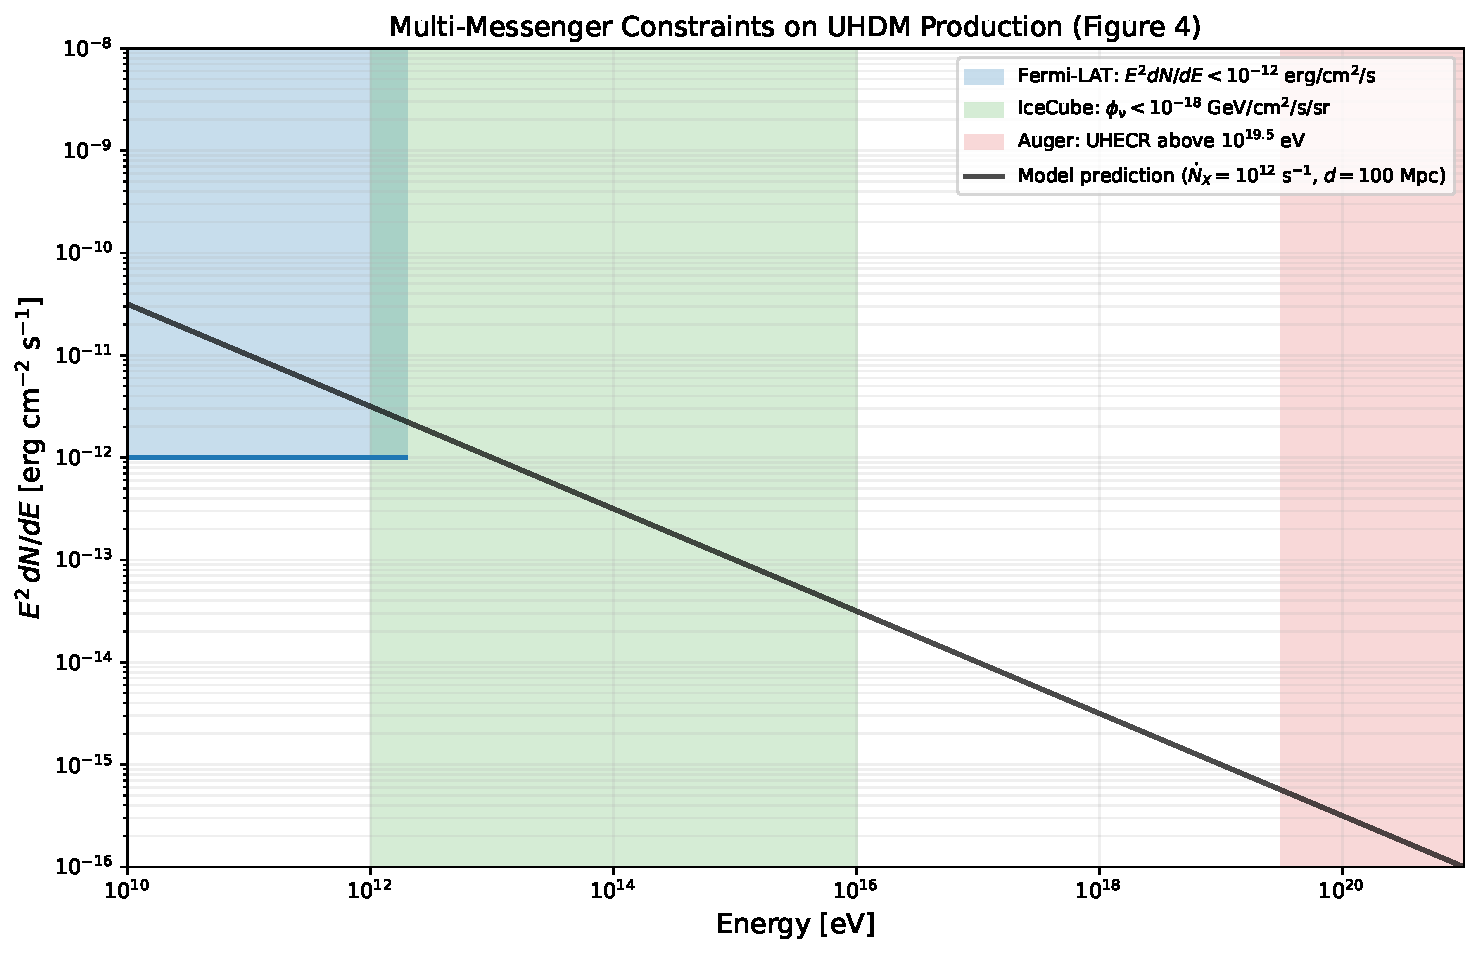
\includegraphics[width=\columnwidth]{../figures/fig4_constraints.pdf}
\caption{Combined multi-messenger constraints.}
\label{fig:constraints}
\end{figure}

\section{Discussion}
[Discussion of results and implications]

\section{Conclusions}
[Summary and future directions]

\begin{acknowledgments}
[Acknowledgments]
\end{acknowledgments}

\bibliography{references}

\end{document}
